% Research roadmap (the user's framework raster, relabelled 2026-10-27 by figs/src/relabel_framework.py). Supplement only, not the method figure.
\begin{figure*}[t]
\centering
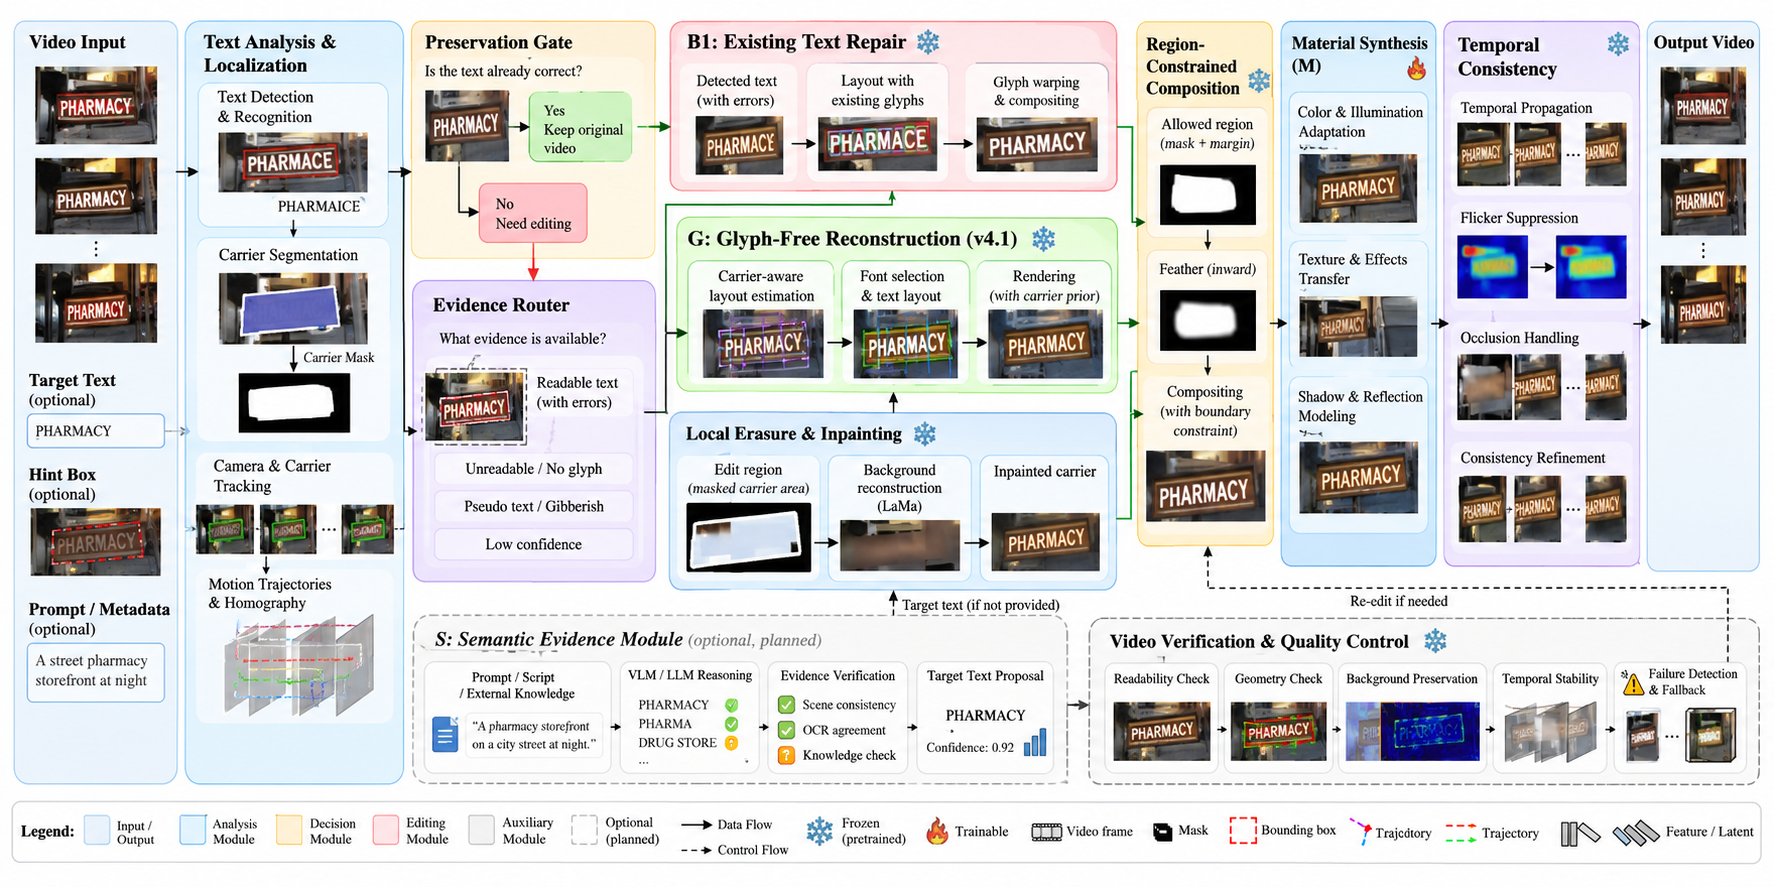
\includegraphics[width=\linewidth]{figs/fig_overview_framework.png}
\caption{\textbf{Research roadmap, not the evaluated method.} The broader framework this work belongs to. Text analysis, the preservation gate, B1 and the region-constrained compositor form the pipeline evaluated in this paper. G, the glyph-free branch, did not pass its sealed cross-generator test and is an exploratory extension (\cref{sec:supp_l3}). The appearance backend is an external pretrained model~\cite{zeng2026steervte}, used only in the Banksy-V hybrid; the constrained fusion (M), the semantic evidence module (S), the evidence router and the verification loop are planned and not claimed, and a trained material generator was a negative result (\cref{sec:exp_neg}). Of the temporal box, only carrier-anchored propagation is part of B1.}
\label{fig:roadmap}
\end{figure*}
